\begin{figure}
	\centering
	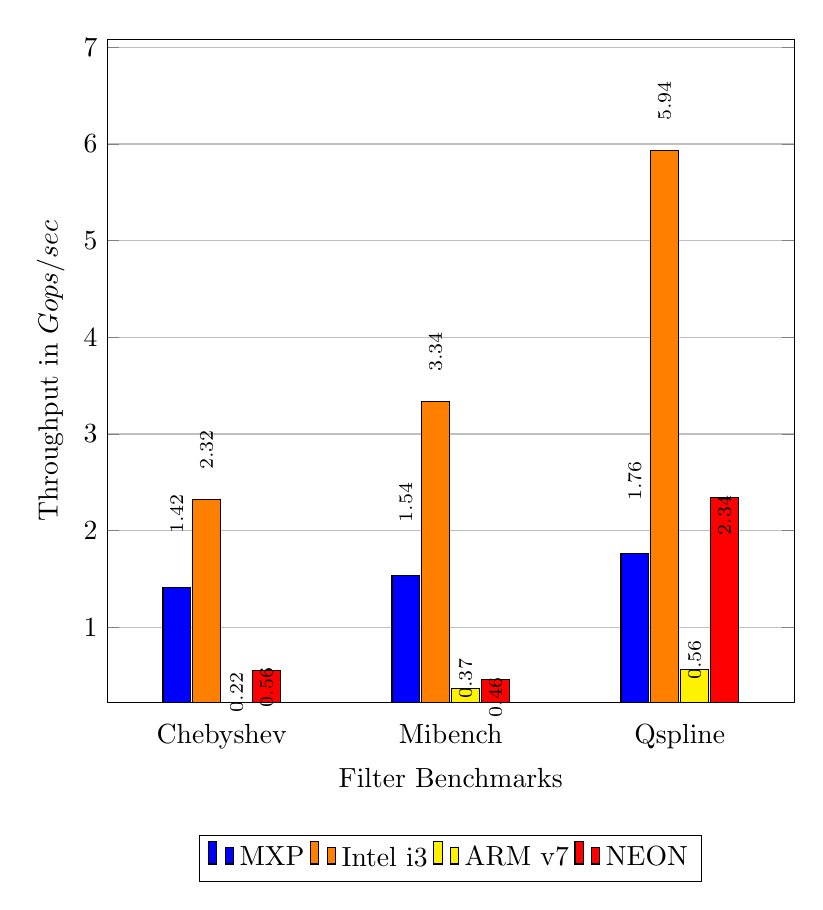
\begin{tikzpicture}
	\begin{axis}[
	width  = 0.85*\textwidth,
	height = 10cm,
	major x tick style = transparent,
	bar width=10pt,
	ymajorgrids = true,
	ylabel = {Throughput in $Gops/sec$},
	xlabel = {Filter Benchmarks},
	symbolic x coords={Chebyshev,Mibench,Qspline},
	xtick = data,
	nodes near coords,
	ybar,
	every node near coord/.append style={rotate=90, anchor=west,font=\scriptsize, xshift=0.25cm},
	scaled y ticks = false,
	enlarge y limits={upper,value=0.2},
	enlarge x limits=0.25,
	ybar=2*\pgflinewidth,
	legend cell align=left,
		legend style={
		at={(.5,-0.2)},
		anchor=north,
		legend columns=-1
		column sep=0.5ex
	}
	]
	\addplot[draw=black,fill=blue, every node near coord/.append style={xshift=.3cm}]
	coordinates {(Chebyshev, 1.417) (Mibench,1.54) (Qspline,1.76)};
	
	\addplot[draw=black,fill=orange]
	coordinates {(Chebyshev, 2.324) (Mibench,3.338) (Qspline,5.935)};
	
	\addplot[draw=black,fill=yellow, every node near coord/.append style={xshift=-0.5cm}]
	coordinates {(Chebyshev, 0.2219) (Mibench,0.3659) (Qspline,0.561)};
	
	\addplot[draw=black,fill=red, every node near coord/.append style={xshift=-0.85cm}]
	coordinates {(Chebyshev, 0.5585) (Mibench,0.460) (Qspline,2.341)};
	
	\legend{MXP,Intel i3,ARM v7,NEON}
	\end{axis}
	\end{tikzpicture}
	\caption{Byte(8-bits) level throughput(Gops/sec) for filter benchmarks }
    \label{filter:1}
\end{figure}